\section{Proceso} 

\begin{itemize}
	\item En el menú Archivo (File) de SQL Server Management,  abriendo el archivo Project.ssmssln.
	\begin{center}
	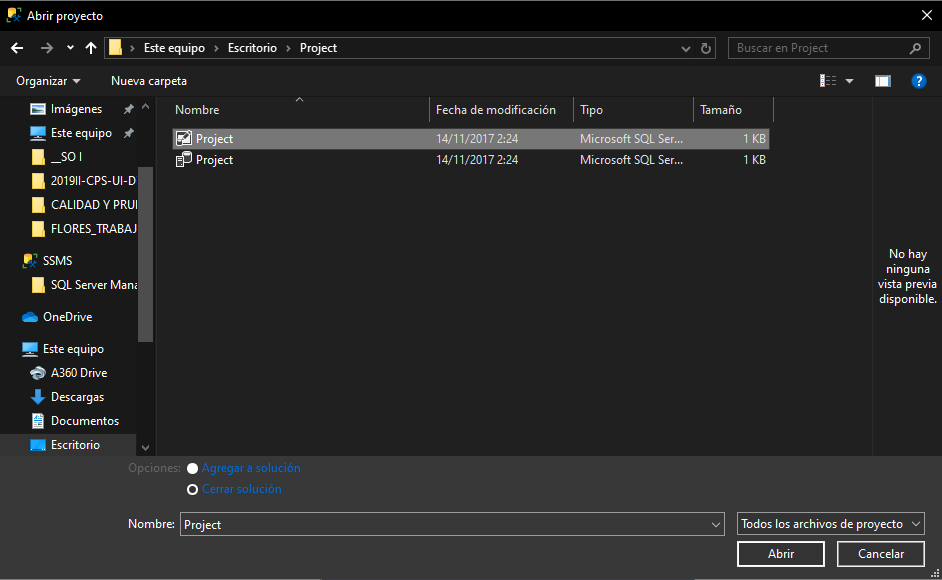
\includegraphics[width=10cm]{./Imagenes/Captura} 
	\end{center}
\end{itemize} 

\begin{itemize}
	\item Obteniendo los datos de la base de datos AdventureWorksLT2017 de Microsoft SQL
	\begin{center}
	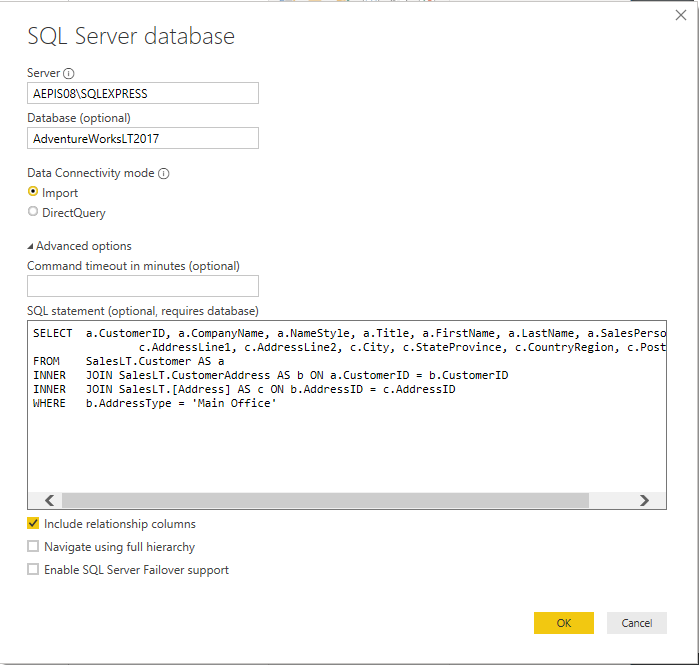
\includegraphics[width=10cm]{./Imagenes/Captura2} 
	\end{center}
\end{itemize} 

\begin{itemize}
	\item  panel Campos (Fields) con las tablas Customers y Sales
	\begin{center}
	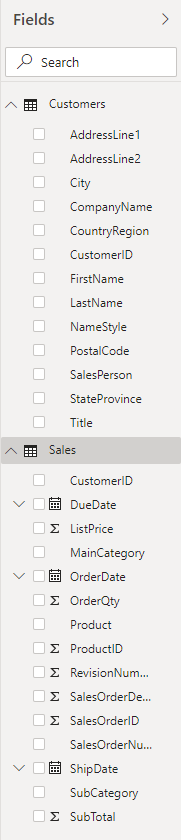
\includegraphics[width=5cm]{./Imagenes/Captura2-1} 
	\end{center}
\end{itemize} 

\begin{itemize}
	\item Eliminando la columna NameStyle de Customers
	\begin{center}
	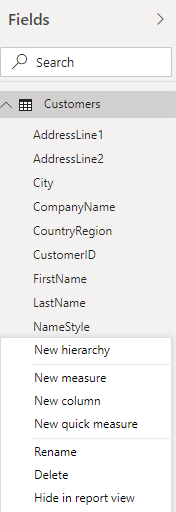
\includegraphics[width=5cm]{./Imagenes/Captura2-2} 
	\end{center}
\end{itemize} 

\begin{itemize}
	\item Eliminando la columna SalesPerson de Customers
	\begin{center}
	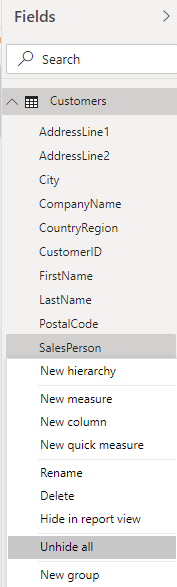
\includegraphics[width=5cm]{./Imagenes/Captura2-3} 
	\end{center}
\end{itemize} 

\begin{itemize}
	\item Ocultando en la vista del reporte CustomerID
	\begin{center}
	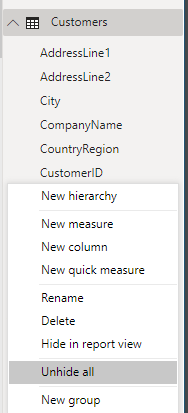
\includegraphics[width=5cm]{./Imagenes/Captura2-4} 
	\end{center}
\end{itemize} 

\begin{itemize}
	\item Categorizando por direccion la columna AddressLine1
	\begin{center}
	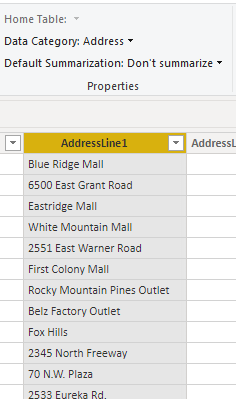
\includegraphics[width=10cm]{./Imagenes/Captura2-5} 
	\end{center}
\end{itemize} 
\begin{itemize}
	\item Categorizando por ciudad la columna City
	\begin{center}
	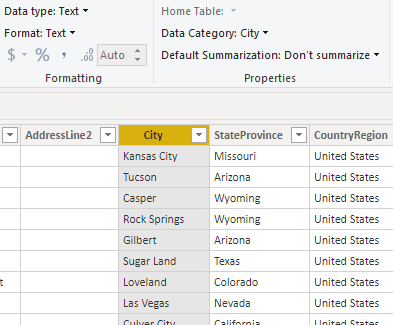
\includegraphics[width=10cm]{./Imagenes/Captura2-6} 
	\end{center}
\end{itemize} 
\begin{itemize}
	\item Categorizando por estado o Provincia la columna StateProvince
	\begin{center}
	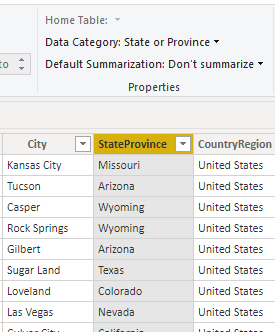
\includegraphics[width=10cm]{./Imagenes/Captura2-7} 
	\end{center}
\end{itemize} 
\begin{itemize}
	\item Categorizando por pais/region la columna CountryRegion
	\begin{center}
	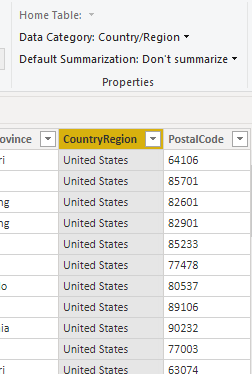
\includegraphics[width=10cm]{./Imagenes/Captura2-8} 
	\end{center}
\end{itemize} 
\begin{itemize}
	\item Categorizando por codigo postal la columna PostalCode
	\begin{center}
	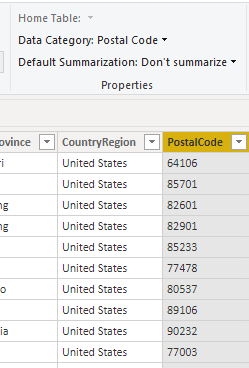
\includegraphics[width=10cm]{./Imagenes/Captura2-9} 
	\end{center}
\end{itemize} 
\begin{itemize}
	\item Creando una cadena de texto para que se muestre la direccion completa
	\begin{center}
	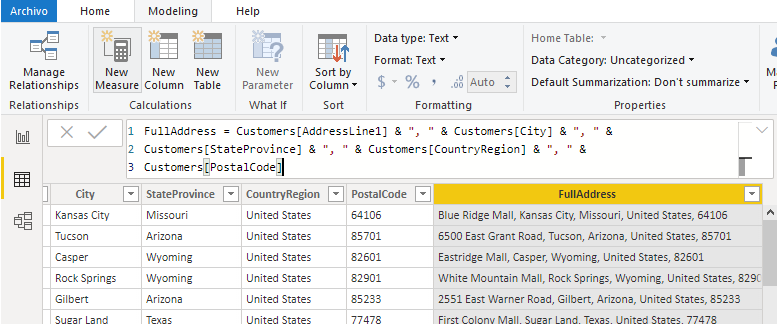
\includegraphics[width=10cm]{./Imagenes/Captura2-10} 
	\end{center}
\end{itemize} 
\begin{itemize}
	\item  Ocultando en la vista del reporte CustomerID de la Sales
	\begin{center}
	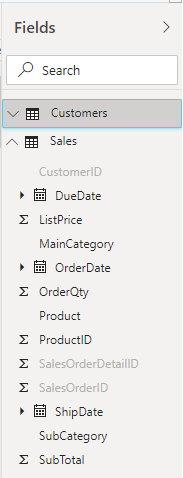
\includegraphics[width=5cm]{./Imagenes/Captura2-11} 
	\end{center}
\end{itemize} 
\begin{itemize}
	\item  Mostrando la multiplicacion de Sales[OrderQty] * Sales[ListPrice]
	\begin{center}
	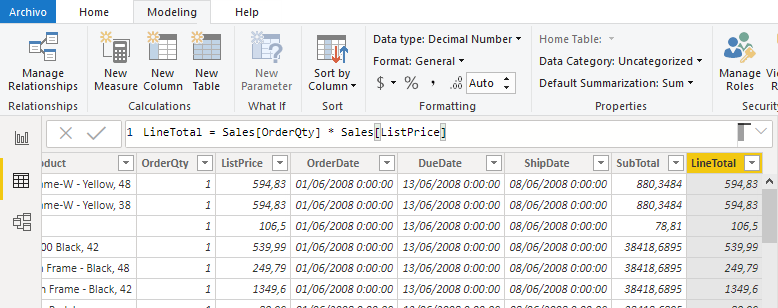
\includegraphics[width=10cm]{./Imagenes/Captura2-12} 
	\end{center}
\end{itemize} 
\begin{itemize}
	\item  Mostrando la multiplicacion la suma de 'Sales'[LineTotal] y multiplicandola por 1.2
	\begin{center}
	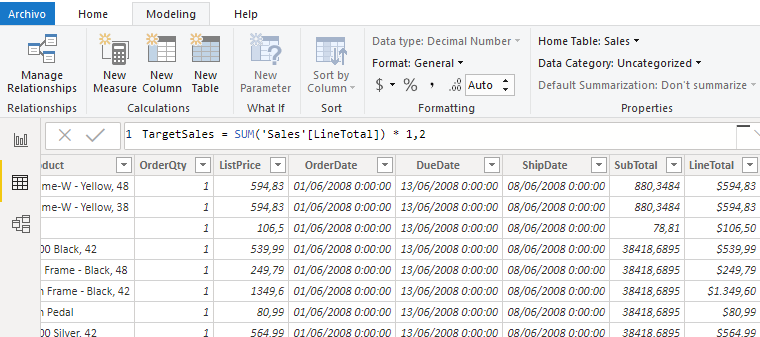
\includegraphics[width=10cm]{./Imagenes/Captura2-13} 
	\end{center}
\end{itemize} 
\begin{itemize}
	\item  Copiando la tabla de States.xlsx a Power Bi y guardandola con el nombre de Sales by State
	\begin{center}
	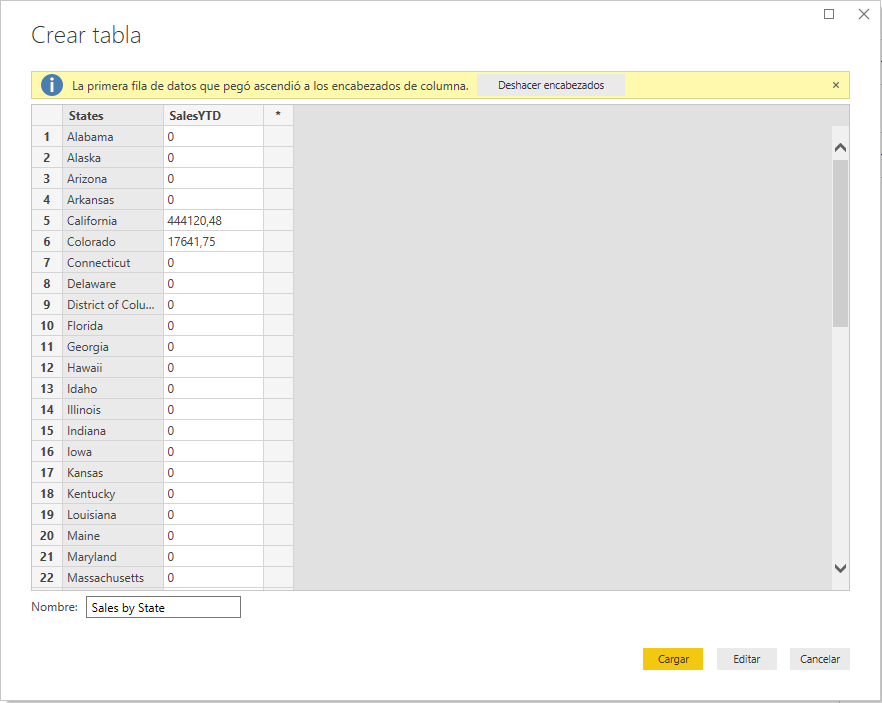
\includegraphics[width=10cm]{./Imagenes/Captura3-1} 
	\end{center}
\end{itemize} 
\begin{itemize}
	\item Obteniendo datos de una web
	\begin{center}
	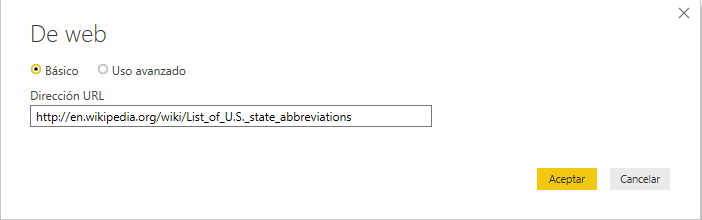
\includegraphics[width=10cm]{./Imagenes/Captura3-2} 
	\end{center}
\end{itemize} 
\begin{itemize}
	\item En el Navegador seleccionamos Codes and abbreviations for U.S. states, territories and other regions para mostrar los datos
	\begin{center}
	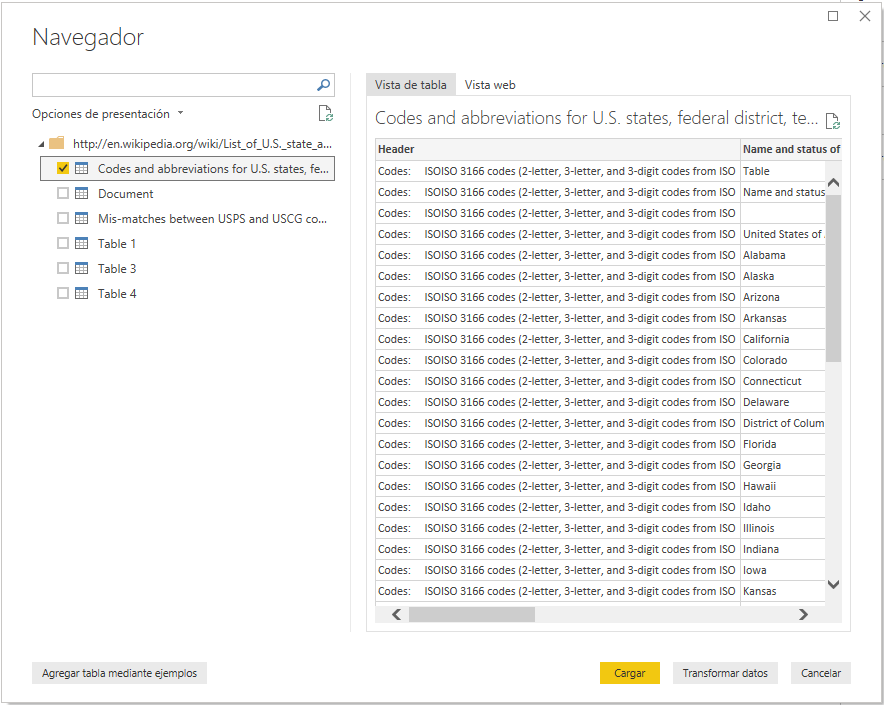
\includegraphics[width=10cm]{./Imagenes/Captura3-3} 
	\end{center}
\end{itemize} 
\begin{itemize}
	\item Seleccionamos Editar consulta
	\begin{center}
	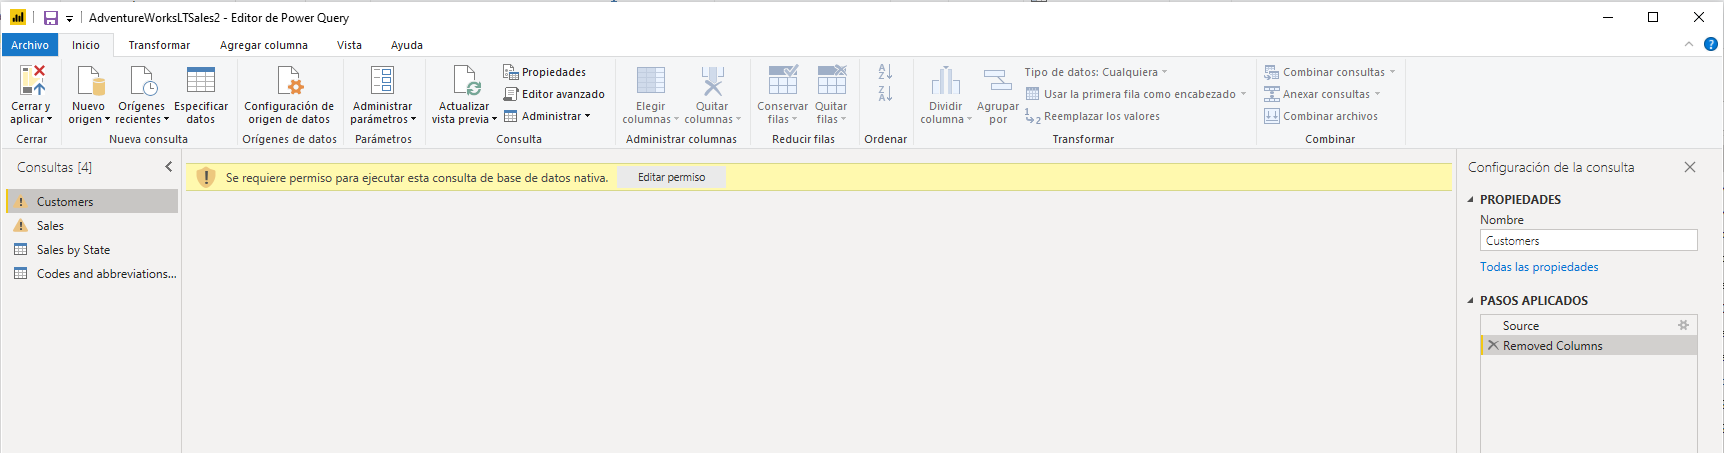
\includegraphics[width=10cm]{./Imagenes/Captura3-4} 
	\end{center}
\end{itemize}
\begin{itemize}
	\item Quitamos 26 filas de Codes and abbreviations for U.S. states, territories and other regions
	\begin{center}
	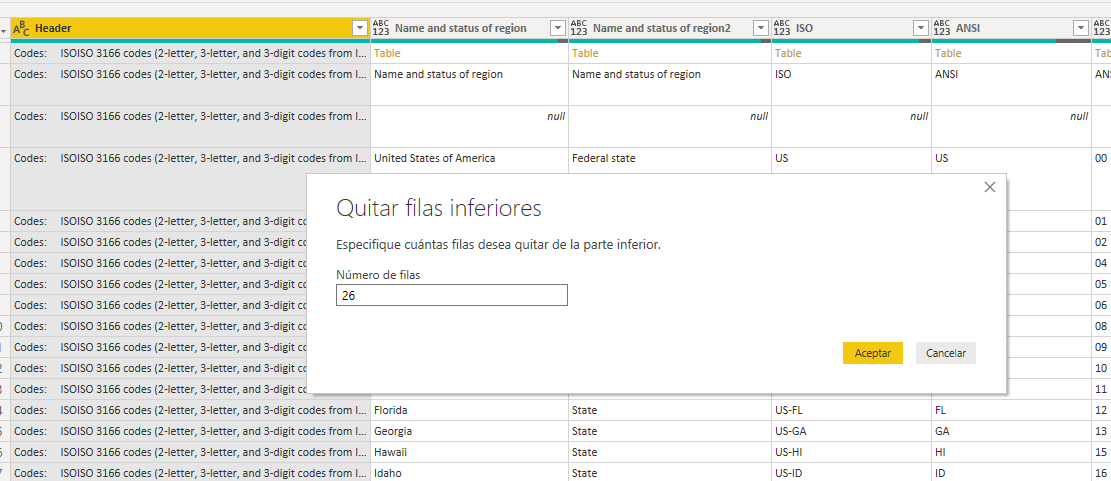
\includegraphics[width=10cm]{./Imagenes/Captura3-5} 
	\end{center}
\end{itemize} 
 \begin{itemize}
	\item Combinamos States de Sales by State con State Name de States with Codes
	\begin{center}
	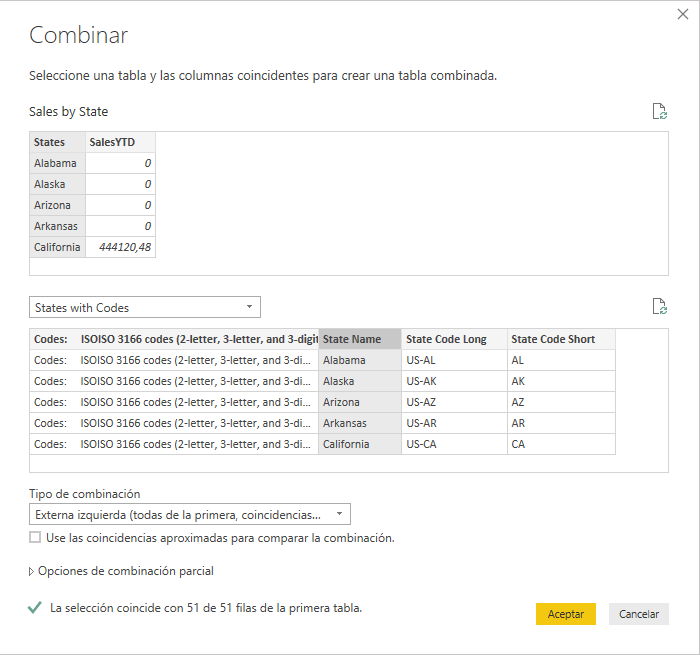
\includegraphics[width=10cm]{./Imagenes/Captura3-8} 
	\end{center}
\end{itemize} 

